\chapter{Champs de jauge, échelles d’interaction et courants faibles chargés}

L’électrodynamique quantique et la chromodynamique quantique semblent très différentes au laboratoire, pourtant toutes deux sont des théories de jauge. En fait, presque toutes les interactions du Modèle standard s’organisent de cette manière. Le mot \emph{jauge} a un sens plus profond, lié à la symétrie locale, mais nous pouvons remettre à plus tard ce formalisme. Pour l’instant, il nous faut une description physique minimale : une théorie de jauge comporte des champs de type Maxwell, des sources conservées, des transformations de symétrie, des bosons de jauge et des règles d’émission et d’absorption de ces bosons.

\section{La théorie de Maxwell comme modèle}

\subsection{Champs et potentiels}

Le champ électromagnétique a six composantes : trois composantes du champ électrique et trois du champ magnétique. On peut encoder les mêmes informations, avec une certaine redondance, dans un quadripotentiel
\begin{equation}
A_\mu=(A_0,\boldsymbol A),
\end{equation}
où \(A_0\) est le potentiel électrostatique et \(\boldsymbol A\) le potentiel vecteur spatial. Dans la limite électrostatique, le champ électrique se déduit du gradient spatial,
\begin{equation}
\boldsymbol E=-\boldsymbol\nabla A_0,
\qquad
\boldsymbol F=q\boldsymbol E,
\end{equation}
tandis que le champ magnétique est donné par
\begin{equation}
\boldsymbol B=\boldsymbol\nabla\times\boldsymbol A.
\end{equation}
Le signe dans la première équation dépend de la définition usuelle du potentiel ; l’explication au tableau porte surtout sur le fait que les champs sont les dérivées des potentiels.
\editorialnote{Pour des champs dépendant du temps, la relation complète est
\(\boldsymbol E=-\boldsymbol\nabla A_0-\partial_t\boldsymbol A\). Dans cette partie, le cours se limite délibérément au cas électrostatique, plus simple.}

\begin{figure}[htbp]
\centering
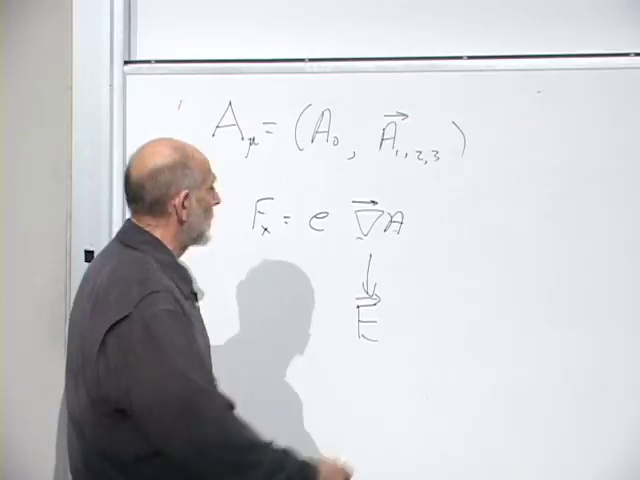
\includegraphics[width=0.62\textwidth]{lecture_05_figure_02.png}
\caption{Le quadripotentiel électromagnétique et sa relation différentielle avec le champ.}
\lectureframe{00:03:33}
\end{figure}

Ainsi, l’électrodynamique admet deux descriptions équivalentes : l’une en termes de \(\boldsymbol E\) et de \(\boldsymbol B\), l’autre en termes de \(A_\mu\).
Cette dernière ne comporte que quatre composantes affichées, car des potentiels différents peuvent décrire les mêmes champs physiques. Cette redondance donne un premier indice sur le sens du mot jauge, même si nous ne l’emploierons pas encore de manière formelle.

\subsection{Ondes et polarisation}

Les équations de Maxwell admettent des solutions sous forme d’ondes. Considérons une onde plane qui se propage dans la direction du vecteur unitaire \(\hat{\boldsymbol k}\). En tout point, les champs électrique et magnétique sont transverses :
\begin{equation}
\boldsymbol E\cdot\hat{\boldsymbol k}=0,
\qquad
\boldsymbol B\cdot\hat{\boldsymbol k}=0,
\qquad
\boldsymbol E\cdot\boldsymbol B=0.
\end{equation}
Dans les unités où \(c=1\), leurs normes sont égales,
\begin{equation}
|\boldsymbol E|=|\boldsymbol B|.
\end{equation}
Pour une onde polarisée linéairement, la direction de \(\boldsymbol E\) spécifie la polarisation. Toute la configuration se propage à la vitesse de la lumière.

La quantification change le langage, mais pas la structure de polarisation. Un quantum de l’onde électromagnétique est un photon. Représenter un photon par un point est forcément trompeur, mais il est utile d’imaginer que ce point porte un petit pointeur transverse qui indique sa polarisation. Une lame quart d’onde ou un autre élément optique peut faire tourner cette polarisation. On peut aussi se représenter, de façon très approximative, un champ statique de Coulomb comme résultant de l’émission et de l’absorption répétées de photons.

\subsection{Sources, flux et conservation}

Les ondes électromagnétiques peuvent se propager dans le vide, mais le champ possède aussi des sources : les charges et les courants électriques. Une charge ponctuelle positive produit un champ électrique radial dirigé vers l’extérieur, proportionnel à \(1/r^2\). Le nombre de lignes de champ qui traversent une sphère entourant la charge est indépendant du rayon de la sphère. Mathématiquement,
\begin{equation}
\oint_{S^2}\boldsymbol E\cdot d\boldsymbol S
=\frac{Q_{\mathrm{enc}}}{\epsilon_0},
\label{eq:l5-gauss}
\end{equation}
en unités SI.

Il ne s’agit pas seulement d’une manière commode de calculer le champ. Les lignes de champ électrique ne peuvent se terminer que sur une charge. Si une charge isolée disparaissait tout simplement, son champ devrait soit disparaître partout à la fois, en violation de la causalité, soit une frontière où le champ manque devrait se propager vers l’extérieur, avec des lignes de champ se terminant dans le vide. Ni l’un ni l’autre n’est possible. La géométrie du flux rend donc naturelle la conservation de la charge : les charges peuvent se déplacer et des charges opposées peuvent s’annihiler, mais la charge nette ne peut disparaître localement sans courant compensateur.

La formulation locale correspondante est l’équation de continuité
\begin{equation}
\partial_t\rho+\boldsymbol\nabla\cdot\boldsymbol J=0.
\label{eq:l5-continuity}
\end{equation}
\editorialnote{~\eqref{eq:l5-continuity} est la forme mathématique locale usuelle de l’argument causal fondé sur le flux, développé oralement dans le cours.}

\subsection{Définition opératoire d’une théorie de jauge}

Nous pouvons maintenant énoncer le schéma général. Une théorie de jauge comprend :
\begin{itemize}
\item des champs de type électrique et de type magnétique ;
\item des ondes qui ressemblent à des ondes lumineuses lorsque les interactions sont suffisamment faibles ;
\item des sources analogues à la charge électrique ;
\item une loi de Gauss reliant le flux à ces sources ;
\item une loi de conservation et une symétrie associée ;
\item des quanta du champ, appelés bosons de jauge ; et
\item une constante de couplage qui régit l’émission et l’absorption.
\end{itemize}
La source n’est pas nécessairement la charge électrique. À titre d’exemple délibérément non physique, imaginons que l’on jauge le nombre baryonique. Les protons et les neutrons ont tous deux un nombre baryonique \(+1\), ils se repousseraient donc par l’intermédiaire d’une nouvelle force de type Coulomb ; un proton et un antiproton s’attireraient. Une telle théorie est concevable mathématiquement, mais la nature ne présente aucun champ de jauge à longue portée observé qui soit couplé au nombre baryonique. La conservation, à elle seule, ne garantit pas l’existence d’une force de jauge.

La charge électrique est bien associée à une symétrie. Pour un champ de matière chargé,
\begin{equation}
\psi(x)\longmapsto e^{i\theta}\psi(x).
\label{eq:l5-u1}
\end{equation}
La symétrie de phase et la conservation de la charge sont deux aspects d’une même structure. Plus tard, nous pourrons faire dépendre \(\theta\) de l’espace-temps et voir pourquoi le potentiel \(A_\mu\) est nécessaire. Ici, la transformation globale suffit à identifier la charge conservée.

\section{La QCD comme exemple non abélien}

\subsection{Triplets, antitriplets et matrice des gluons}

En chromodynamique quantique, un champ de quarks porte un indice de couleur \(i\in\{r,g,b\}\) et se transforme selon la représentation fondamentale de \(SU(3)\) :
\begin{equation}
q'_i=U_{ij}q_j,
\qquad
U^\dagger U=\boldsymbol 1,
\qquad
\det U=1.
\label{eq:l5-q-transform}
\end{equation}
Il s’agit d’une rotation dans un espace complexe de couleur à trois dimensions, et non d’une rotation de l’espace ordinaire. La représentation à trois composantes est aussi appelée représentation définissante.

Les champs d’antiparticules sont représentés par les variables complexes conjuguées. En prenant le complexe conjugué de l’équation~\eqref{eq:l5-q-transform}, on obtient
\begin{equation}
q_i^{\prime *}=U_{ij}^*q_j^*.
\label{eq:l5-antiquark-transform}
\end{equation}
Les quarks se transforment donc selon \(\boldsymbol 3\), tandis que les antiquarks se transforment selon \(\bar{\boldsymbol 3}\).

\begin{figure}[htbp]
\centering
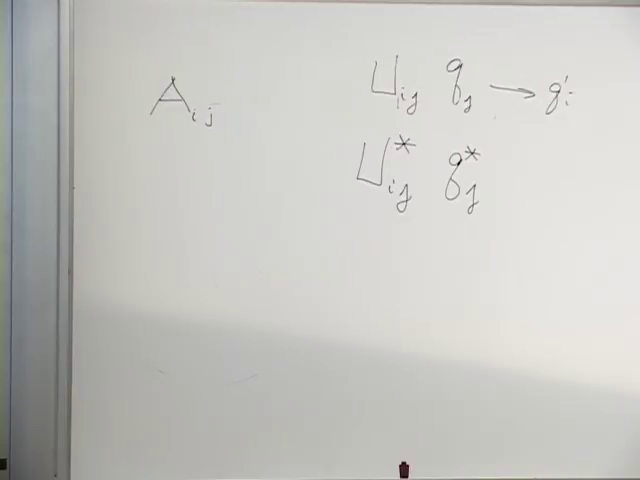
\includegraphics[width=0.62\textwidth]{lecture_05_figure_03.png}
\caption{La transformation fondamentale et la transformation complexe conjuguée en antitriplet.}
\lectureframe{00:18:47}
\end{figure}

\begin{classroomqa}\audiencequestion{Combien y a-t-il de matrices \(U\) : sept, huit ou neuf ?
--\lecturetimestamp{00:19:37}}\lecturerresponse{Les éléments du groupe \(U\) sont en nombre infini. Le nombre fini que l’on compte est celui des générateurs indépendants ; il est égal à huit pour \(SU(3)\). Une matrice générale \(3\times3\) comporte neuf positions, mais la condition d’unitarité spéciale ne laisse que huit directions continues.}\end{classroomqa}

Le champ des gluons peut s’écrire sous la forme d’une matrice sans trace \(A_{ij}\). Un indice se transforme comme celui d’un quark et l’autre comme celui d’un antiquark ; sa structure de couleur correspond donc à
\begin{equation}
\boldsymbol 3\otimes\bar{\boldsymbol 3}
=\boldsymbol 1\oplus\boldsymbol 8.
\end{equation}
La QCD conserve l’octet sans trace,
\begin{equation}
A_{ii}=\operatorname{tr}A=0,
\end{equation}
et écarte le singulet. C’est pourquoi la QCD comporte huit gluons, et non neuf. Plus généralement, \(SU(N)\) possède
\begin{equation}
N^2-1
\end{equation}
générateurs et autant de champs de bosons de jauge.

Le photon est neutre vis-à-vis de la charge électrique \(U(1)\) : faire tourner la phase d’un électron ne transforme pas le photon en un autre photon. Les gluons sont différents. Un gluon porte une couleur et une anticouleur ; il se transforme donc selon la représentation adjointe. Une combinaison rouge--anti-bleu, par exemple, n’est pas un singulet de couleur, même si elle contient une couleur et une anticouleur.

\subsection{Flux des indices et auto-interaction}

On peut comprendre la règle d’interaction en suivant les indices. Schématiquement, un quark de couleur \(i\) peut devenir un quark de couleur \(j\) en émettant un gluon qui porte le flux de couleur correspondant :
\begin{equation}
q_i\longrightarrow q_j+A_{ij}.
\label{eq:l5-quark-gluon-vertex}
\end{equation}
Le placement précis de \(i\) et de \(j\) dépend de la convention choisie pour les flèches ; le contenu invariant est que tout indice entrant dans un sommet doit se poursuivre sur une autre ligne. Aucun indice de couleur ne disparaît.

Cette règle vaut dans toute théorie de jauge \(SU(N)\). La matière fondamentale porte un indice, la matière antifondamentale un indice conjugué et un boson de jauge en porte un de chaque type. Les noms physiques peuvent varier, mais la structure des indices reste la même.

Comme un gluon porte lui-même une couleur, il peut émettre un autre gluon. Un gluon \(A_{ij}\) peut se scinder en passant par un indice intermédiaire \(k\), schématiquement :
\begin{equation}
A_{ij}\longrightarrow A_{ik}+A_{kj}.
\label{eq:l5-three-gluon-index}
\end{equation}
Ce n’est pas un sommet de Yang--Mills complet, mais il montre le flux de couleur. Rien de semblable ne se produit pour les photons en électrodynamique ordinaire. Les gluons exercent donc des forces les uns sur les autres, et la dynamique des champs non abéliens est bien plus complexe que la théorie linéaire de Maxwell.

Une conséquence qualitative est le confinement. Les lignes de flux de couleur ne peuvent pas se terminer ; leur auto-interaction les rassemble en un tube reliant un quark à un antiquark. Le tube porte une énergie approximativement constante par unité de longueur :
\begin{equation}
V(R)\simeq \sigma R.
\end{equation}
Éloigner davantage ses extrémités emmagasine donc plus d’énergie, au lieu de libérer une couleur isolée. C’est l’image de la colle gluante : le champ lui-même empêche les constituants colorés de s’échapper sous forme de particules libres.

\section{Couplages et sens de « fort » ou « faible »}

\subsection{La charge comme amplitude d’émission}

Une théorie de jauge a tout de même besoin d’une constante de couplage. En QED, la charge de l’électron \(e\) est le coefficient associé à un sommet électron--photon. C’est une amplitude, et les probabilités sont les carrés des amplitudes. Pour se représenter concrètement la situation, imaginons qu’un électron rapide soit brusquement arrêté dans un tube cathodique. La probabilité d’émettre un photon est proportionnelle à \(e^2\), les facteurs conventionnels étant incorporés à la constante de structure fine,
\begin{equation}
\alpha=\frac{e^2}{4\pi\hbar c}
\simeq \frac{1}{137}.
\label{eq:l5-alpha}
\end{equation}
Dans les unités naturelles \(\hbar=c=1\), le couplage est sans dimension. Une échelle d’un pour cent pour une émission élémentaire signifie que l’électromagnétisme est faible au sens perturbatif : la plupart des électrons arrêtés ne libèrent pas chacun une gerbe de photons durs.

\subsection{Les unités naturelles relient énergie, temps et distance}

Posons
\begin{equation}
c=1,
\qquad
\hbar=1.
\end{equation}
Le temps et la distance ont alors les mêmes unités, tandis que l’énergie s’exprime en unités inverses :
\begin{equation}
E=\hbar\omega\longrightarrow E=\omega\sim\frac1t,
\qquad
x\sim t\sim\frac1E.
\end{equation}
Les grandes énergies sondent de petites distances et de courtes durées.

Pour se faire une idée des ordres de grandeur,
\begin{equation}
1\ {\rm eV}^{-1}
=\frac{\hbar c}{1\ {\rm eV}}
\simeq 1.97\times10^{-7}\ {\rm m}.
\end{equation}
Une longueur atomique de l’ordre de \(10^{-10}\ {\rm m}\) correspond donc approximativement à l’inverse d’un kiloelectronvolt. Il s’agit de conversions d’ordre de grandeur, et non de mesures spectroscopiques de précision.

\subsection{La hiérarchie à l’intérieur d’un atome}

Pour un atome typique, prenons
\begin{equation}
R_{\rm atom}\sim10^{-10}\ {\rm m}.
\end{equation}
La lumière parcourt cette distance en
\begin{equation}
t_{\rm transit}^{\rm atom}\sim10^{-18}\ {\rm s}.
\end{equation}
Dans un atome léger, toutefois, l’électron se déplace à une fraction seulement de la vitesse de la lumière. Dans le modèle de Bohr, \(v/c\sim\alpha\), de sorte que la période orbitale typique est plus longue :
\begin{equation}
t_{\rm orbit}^{\rm atom}\sim10^{-16}\ {\rm s}.
\end{equation}

Un atome excité met encore plus longtemps à rayonner :
\begin{equation}
t_{\rm decay}^{\rm atom}\sim10^{-9}\ {\rm s}
\end{equation}
Il s’agit d’une estimation approximative, à l’échelle du cours. Le tableau physique comporte deux facteurs de suppression. La force électromagnétique ne produit qu’une accélération modeste, et un électron accéléré présente une autre faible probabilité d’émission, gouvernée par \(\alpha\). La petitesse de la constante de structure fine engendre donc une hiérarchie entre les durées de transit, de révolution orbitale et de désintégration radiative.

\subsection{L’absence de hiérarchie dans un hadron}

Un hadron est un système lié, analogue à un atome, constitué de quarks et de gluons, mais son échelle est bien plus petite :
\begin{equation}
R_{\rm hadron}\sim10^{-15}\ {\rm m},
\qquad
t_{\rm transit}^{\rm hadron}\sim10^{-23}\ {\rm s}.
\end{equation}
Les quarks traversent le hadron sur une échelle de temps pratiquement identique, et les hadrons excités qui se désintègrent par interaction forte vivent eux aussi environ
\begin{equation}
t_{\rm orbit}^{\rm hadron}
\sim t_{\rm decay}^{\rm hadron}
\sim10^{-23}\ {\rm s}.
\end{equation}
Un hadron frappé peut vibrer et émettre un pion presque aussi vite que le permet la causalité. Il n’existe pas de séparation de sept ou neuf ordres de grandeur comme à l’intérieur d’un atome.

\begin{classroomqa}\audiencequestion{La relativité restreinte implique-t-elle qu’un hadron ne peut pas se désintégrer beaucoup plus vite que son temps de traversée par la lumière ?
\lecturetimestamp{00:47:15}}\lecturerresponse{C’est une manière raisonnable d’énoncer la borne en ordre de grandeur. Les désintégrations fortes se produisent à peu près aussi vite que le permet la taille du système ; aucun petit couplage ni autre facteur de suppression important ne les ralentit.}\end{classroomqa}

Le couplage fort correspondant est donc bien supérieur à \(\alpha\). À titre d’illustration, à l’échelle hadronique, le cours donne
\begin{equation}
\alpha_{\rm QCD}\sim0.2,
\end{equation}
une valeur beaucoup plus proche de l’unité que \(1/137\). C’est l’origine dynamique de l’ancien nom « \emph{interactions fortes} ».
\editorialnote{\(\alpha_s\) varie avec l’énergie, ce n’est donc pas une valeur fixe. La valeur citée est illustrative et dépend de l’échelle, comme le cours le précise.}

\begin{classroomqa}\audiencequestion{L’analogue fort s’appelle-t-il simplement la constante de force forte ?
\lecturetimestamp{00:48:17}}\lecturerresponse{On l’appelle conventionnellement \(\alpha_{\rm QCD}\), ou plus souvent \(\alpha_s\). Pour le couplage électromagnétique, on dit généralement simplement \(\alpha\), bien que l’on puisse utiliser \(\alpha_{\rm QED}\) lorsque les deux couplages apparaissent dans la même discussion.}\end{classroomqa}

\begin{classroomqa}\audiencequestion{Dans un article, distinguerait-on un couplage électromagnétique nu de sa valeur mesurée, écrantée ?
\lecturetimestamp{00:48:38}}\lecturerresponse{Oui. On parle de couplage nu et de couplage renormalisé. La polarisation du vide fait dépendre le couplage effectif de l’échelle à laquelle on le mesure.}\end{classroomqa}

\section{Le problème de la désintégration faible}

Les interactions faibles ont été nommées ainsi en raison de leurs très longues durées de désintégration. Elles sont généralement plus lentes que les désintégrations fortes et peuvent même prendre plus de temps que le rayonnement atomique. Le plus ancien exemple est la désintégration bêta nucléaire.

\subsection{Désintégration bêta du neutron}

Un neutron libre se désintègre selon
\begin{equation}
n\longrightarrow p+e^-+\bar\nu_e.
\label{eq:l5-neutron-decay-intro}
\end{equation}
Le cours utilise une durée de vie d’environ douze minutes, démesurément longue par rapport à \(10^{-23}\ {\rm s}\). Les valeurs de précision actuelles n’ont pas d’importance pour l’argument.

Une partie de cette lenteur est d’origine cinématique. En gros,
\begin{equation}
\begin{aligned}
m_n&\simeq940\ {\rm MeV},
&
m_p&\simeq939\ {\rm MeV},
\\
m_e&\simeq0.5\ {\rm MeV}.
\end{aligned}
\end{equation}
Seule une infime fraction de l’énergie de masse au repos du neutron est disponible sous forme d’énergie cinétique. Si le neutron était plus léger que la somme des masses au repos des produits finaux, la désintégration serait impossible. S’il se situait à peine au-dessus du seuil, l’espace de phase disponible serait minuscule et la désintégration serait lente. Mais l’espace de phase ne peut à lui seul expliquer une durée de vie de plusieurs minutes.

\subsection{Le pion chargé écarte l’explication par le seuil}

Considérons aussi
\begin{equation}
\pi^-\longrightarrow e^-+\bar\nu_e
\end{equation}
et le processus conjugué de charge. Le pion possède une énergie largement supérieure au seuil du canal électronique, pourtant sa durée de vie faible est toujours de l’ordre de la nanoseconde, au lieu des \(10^{-23}\) secondes typiques des processus hadroniques. Un canal analogue faisant intervenir un muon deviendra bientôt important. Le problème est donc intrinsèque à l’interaction faible, et ne tient pas simplement aux masses presque dégénérées du neutron.

\editorialnote{\(26\ {\rm ns}\), et le canal dominant est \(\pi^-\to\mu^-\bar\nu_\mu\). Le canal électronique est supprimé par l’hélicité. Le cours commence par le canal électronique, car c’est le plus simple pour tenir le compte des particules, puis revient au canal dominant avec un muon.}

Le terme désintégration bêta vient de l’usage historique du nom « rayons bêta » pour désigner les électrons émis. Les exemples du pion et du neutron font intervenir la même interaction de courant chargé, même si leur cinématique diffère fortement.

\section{Tableau des quarks et des leptons}

\subsection{La couleur agit verticalement}

Disposons les six saveurs de quarks en trois paires,
\begin{equation}
(u,d),\qquad(c,s),\qquad(t,b),
\end{equation}
puis plaçons une copie rouge, verte et bleue de chaque quark dans des lignes distinctes. La couleur \(SU(3)\) agit verticalement : elle transforme l’une en l’autre les versions rouge, verte et bleue d’un quark up, et effectue simultanément la même rotation de couleur pour les quarks down, charm, strange, top et bottom. Elle ne transforme pas un quark up en quark down.

\subsection{L’isospin faible agit horizontalement}

La symétrie faible agit dans l’autre direction. Elle mélange chaque paire de saveurs voisines :
\begin{equation}
Q_1=\begin{pmatrix}u\\d\end{pmatrix},
\qquad
Q_2=\begin{pmatrix}c\\s\end{pmatrix},
\qquad
Q_3=\begin{pmatrix}t\\b\end{pmatrix}.
\label{eq:l5-quark-doublets}
\end{equation}
Les quarks de type up ont une charge \(+2/3\), et les quarks de type down une charge \(-1/3\) ; la charge change donc d’une unité au sein de chaque paire.
\editorialnote{Le cours indique brièvement qu’un quark down a une charge \(-2/3\). La soustraction qui l’entoure et tous les processus qui suivent impliquent la valeur usuelle \(-1/3\), utilisée ici.}

Puisque la symétrie agit sur des doublets, le groupe naturel est \(SU(2)\). Il agit sur chaque copie de couleur de chaque doublet de quarks sans changer la couleur.

Il existe aussi une quatrième ligne de particules qui ne portent pas de couleur et n’interagissent donc pas avec les gluons : les leptons. Ils forment trois autres doublets,
\begin{equation}
L_e=\begin{pmatrix}\nu_e\\e^-\end{pmatrix},
\qquad
L_\mu=\begin{pmatrix}\nu_\mu\\\mu^-\end{pmatrix},
\qquad
L_\tau=\begin{pmatrix}\nu_\tau\\\tau^-\end{pmatrix}.
\label{eq:l5-lepton-doublets}
\end{equation}
Les neutrinos sont électriquement neutres ; l’électron, le muon et le tau ont une charge \(-1\). Là encore, les deux membres diffèrent d’une unité de charge électrique. L’électron, le muon et le tau ont les mêmes nombres quantiques de jauge, mais des masses différentes, tout comme les trois générations de quarks de type up ou down reproduisent le même schéma de charge.

\begin{figure}[htbp]
\centering
\includegraphics[width=0.82\textwidth]{lecture_05_figure_05.png}
\caption{Le tableau au tableau : la couleur agit entre les lignes rouge, bleue et verte, tandis que l’\(SU(2)\) faible relie les colonnes de saveurs appariées et la ligne des leptons.}
\lectureframe{01:03:35}
\end{figure}

À ce stade, qualifier les leptons de quatrième couleur n’est qu’une analogie. Ils occupent une quatrième ligne du tableau des doublets faibles, mais la QCD ordinaire \(SU(3)\) ne transforme pas les quarks en leptons.

\section{Construction des bosons faibles chargés}

\subsection{Nombres quantiques des bosons chargés}

Les bosons de jauge portent les propriétés de transformation nécessaires pour passer d’un membre d’un doublet à l’autre. Commençons par la paire leptonique \(e^-\bar\nu_e\). Sa charge électrique est \(-1\) ; le boson de jauge chargé correspondant est donc appelé \(W^-\) :
\begin{equation}
W^-\sim e^-\bar\nu_e.
\end{equation}
On retrouve les mêmes nombres quantiques à partir d’un quark down et d’un antiquark up :
\begin{equation}
W^-\sim d\bar u.
\end{equation}
Le symbole \(\sim\) signifie : a les mêmes nombres quantiques de jauge pertinents que. Il ne signifie pas que le \(W\) est littéralement un état lié de ces particules. L’antiparticule comporte les combinaisons conjuguées,
\begin{equation}
W^+\sim e^+\nu_e\sim\bar d u.
\end{equation}

Les sommets faibles chargés comprennent
\begin{align}
e^-&\longrightarrow\nu_e+W^-,
&
\mu^-&\longrightarrow\nu_\mu+W^-,
\label{eq:l5-lepton-w}\\
d&\longrightarrow u+W^-,
&
s&\longrightarrow c+W^-,
\label{eq:l5-quark-w}
\end{align}
avec des transitions analogues pour la troisième génération lorsque la cinématique le permet. Le boson de jauge réalise dynamiquement le même mélange horizontal que la symétrie réalise sur le doublet.

\begin{classroomqa}\audiencequestion{La conservation de la charge impose que le boson émis ait une charge \(-1\), mais pourquoi les transitions de l’électron, du quark down et du quark strange font-elles toutes intervenir la même particule ?
\lecturetimestamp{01:12:56}}\lecturerresponse{C’est un fait empirique encodé par la symétrie faible commune. La nature aurait pu attribuer de façon cohérente un boson de type \(W\) différent à chaque famille, ou aux quarks et aux leptons séparément. Au lieu de cela, un seul \(SU(2)\) agit simultanément sur tous les doublets, et les mêmes bosons de jauge chargés médiatisent toutes ces transitions.}\end{classroomqa}

\subsection{Lire un sommet et inverser une réaction}

Un sommet unique représente toute une famille de processus. Inverser une ligne entrante en ligne sortante transforme une particule en son antiparticule ; inverser une ligne \(W^-\) donne un \(W^+\). On peut donc lire un sommet comme une émission, une absorption, une désintégration, une annihilation ou la réaction inverse, à condition de suivre de manière cohérente la charge, la quantité de mouvement et tous les nombres quantiques pertinents.

\begin{classroomqa}\audiencequestion{Peut-on inverser les flèches et les lignes de ces sommets faibles ?
\lecturetimestamp{01:14:51}}\lecturerresponse{Oui. On peut croiser une ligne pour la faire passer de l’état final à l’état initial, ou inversement, mais la particule devient alors son antiparticule. Le même sommet local décrit par conséquent de nombreuses réactions orientées différemment.}\end{classroomqa}

\begin{classroomqa}\audiencequestion{Écrire un \(W^-\) avec des lignes strange et charm signifie-t-il que le boson est littéralement un quark strange lié à un antiquark charm ?
\lecturetimestamp{01:15:43}}\lecturerresponse{Non. Le suivi des lignes indique seulement que le \(W^-\) porte le changement de nombres quantiques entre ces colonnes. Si l’on lit le diagramme comme une désintégration, un \(W^-\) suffisamment énergétique peut produire un quark strange et un antiquark charm ; il n’est pas composé de ces particules.}\end{classroomqa}

\begin{classroomqa}\audiencequestion{Un électron et un antineutrino peuvent-ils former un \(W\), qui produit ensuite une paire de quarks ?
\lecturetimestamp{01:17:22}}\lecturerresponse{Exactement. Si l’énergie dans le centre de masse est suffisante, les leptons initiaux peuvent former l’état intermédiaire de courant chargé, qui peut ensuite se manifester par un canal de quarks autorisé. Ce sont les mêmes deux sommets que ceux de la désintégration, lus dans une autre orientation.}\end{classroomqa}

\subsection{Le troisième boson manquant}

Le groupe \(SU(2)\) possède trois générateurs, et donc trois champs de jauge. Jusqu’ici, nous n’avons représenté que \(W^+\) et \(W^-\). Un troisième champ, électriquement neutre, doit correspondre à des combinaisons diagonales telles que celles associées aux nombres quantiques électron--positron et neutrino--antineutrino. Il reste délibérément en arrière-plan. Son lien avec le boson \(Z\) physique et le photon nécessite le mélange électrofaible, qui sera abordé plus tard.

\begin{classroomqa}\audiencequestion{A-t-on soupçonné l’existence des forces faible et forte à des époques différentes ?
\lecturetimestamp{01:24:11}}\lecturerresponse{Leurs racines expérimentales sont apparues ensemble dans les débuts de l’étude de la radioactivité. La désintégration alpha a révélé la physique nucléaire et celle des interactions fortes, la désintégration bêta a révélé l’interaction faible, et la désintégration gamma a émis des photons électromagnétiques. À l’époque de Becquerel, on disposait déjà de ces trois indices, bien avant l’apparition des théories modernes des champs.}\end{classroomqa}

\section{Exemples de désintégrations par courant chargé}

\subsection{Désintégration du pion}

Le pion de charge négative a pour contenu en quarks de valence
\begin{equation}
\pi^-=d\bar u.
\end{equation}
Ces nombres quantiques permettent une annihilation en un \(W^-\), qui peut ensuite produire un lepton chargé et l’antineutrino correspondant :
\begin{align}
\pi^-&\longrightarrow W^{-*}
\longrightarrow e^-+\bar\nu_e,
\label{eq:l5-pion-electron}\\
\pi^-&\longrightarrow W^{-*}
\longrightarrow \mu^-+\bar\nu_\mu.
\label{eq:l5-pion-muon}
\end{align}
L’astérisque rappelle que le \(W\) intermédiaire est virtuel. Le second canal est le canal dominant.

\begin{figure}[htbp]
\centering
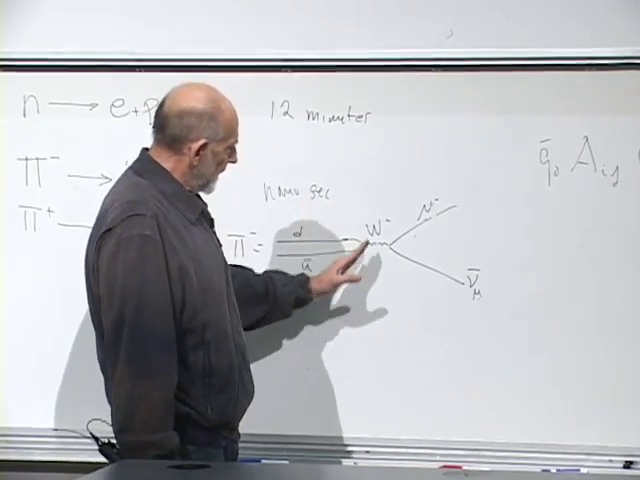
\includegraphics[width=0.72\textwidth]{lecture_05_figure_04.png}
\caption{Un pion \(d\bar u\) s’annihile en un \(W^-\) virtuel, puis donne un lepton chargé et l’antineutrino correspondant.}
\lectureframe{01:19:38}
\end{figure}

\begin{classroomqa}\audiencequestion{S’agit-il vraiment d’un diagramme de Feynman, même si le temps a été représenté horizontalement plutôt que verticalement ?
\lecturetimestamp{01:20:21}}\lecturerresponse{Oui. L’orientation du temps sur la page est une convention. Dès que l’on choisit une direction pour représenter le temps et que l’on interprète toutes les flèches de manière cohérente, le dessin contient les mêmes informations sur les interactions.}\end{classroomqa}

\begin{classroomqa}\audiencequestion{Peut-on lire le diagramme comme une réaction chimique réversible plutôt que comme une désintégration irréversible à sens unique ?
\lecturetimestamp{01:21:35}}\lecturerresponse{Le processus inverse est permis. Un pion produit dans le vide se désintègre parce que les particules émises s’éloignent et ne se recombinent pas en temps normal. Mais si l’on fait entrer en collision un muon et un antineutrino avec l’énergie et la quantité de mouvement voulues, l’amplitude de formation du pion par l’interaction inverse est non nulle.}\end{classroomqa}

\subsection{Énergie et état intermédiaire virtuel}

Pour un pion au repos,
\begin{equation}
m_\pi\simeq140\ {\rm MeV},
\qquad
m_\mu\simeq106\ {\rm MeV},
\qquad
m_\nu\approx0
\end{equation}
à la précision pertinente ici. L’énergie restante devient l’énergie cinétique des particules émises. La conservation de la quantité de mouvement impose
\begin{equation}
\boldsymbol p_\mu+\boldsymbol p_{\bar\nu}=0,
\end{equation}
que les deux particules partent en directions opposées dans le référentiel de repos du pion.

\begin{classroomqa}\audiencequestion{Comment l’énergie peut-elle se conserver si le \(W\) intermédiaire est bien plus lourd que le pion ?
\lecturetimestamp{01:25:08}}\lecturerresponse{Seules les particules initiales et finales doivent être sur leur couche de masse. La quadri-impulsion se conserve à chaque sommet, mais une ligne interne virtuelle n’a pas besoin de satisfaire à \(E^2=\boldsymbol p^2+m_W^2\). Plus l’écart à la couche de masse est important, plus le propagateur correspondant supprime le processus.\editorialnote{Le cours emploie le langage traditionnel de l’incertitude énergie--temps et dit que l’état intermédiaire peut brièvement violer la conservation de l’énergie. La formulation moderne précise est celle de la réponse : la quantité de mouvement-énergie se conserve, mais une ligne interne virtuelle n’a pas à satisfaire à la condition de couche de masse d’une particule réelle.}}\end{classroomqa}

\subsection{Désintégration du muon}

Un muon peut d’abord se transformer en son propre neutrino en émettant un \(W^-\) virtuel :
\begin{equation}
\mu^-\longrightarrow\nu_\mu+W^{-*}.
\end{equation}
Le boson virtuel produit ensuite un électron et un antineutrino électronique :
\begin{equation}
\mu^-\longrightarrow
\nu_\mu+e^-+\bar\nu_e.
\label{eq:l5-muon-decay}
\end{equation}
Il s’agit d’un processus purement leptonique. Le muon est environ deux cents fois plus lourd que l’électron ; les masses au repos des produits finaux laissent donc une ample marge pour l’énergie cinétique.

\begin{figure}[htbp]
\centering
\includegraphics[width=0.72\textwidth]{lecture_05_figure_06.png}
\caption{Désintégration du muon par l’intermédiaire d’un boson faible chargé virtuel.}
\lectureframe{01:29:24}
\end{figure}

\begin{classroomqa}
\audiencequestion{La particule neutre émise avec l’électron est-elle un antineutrino ?
\lecturetimestamp{01:29:06}}
\lecturerresponse{Oui. L’état final complet contient un neutrino muonique, un antineutrino électronique et l’électron. Conserver les indices de saveur permet de ne pas confondre les deux particules neutres.}
\end{classroomqa}

L’électron ne peut pas inverser cette désintégration dans le vide, car il est plus léger que le muon. Le tau, plus lourd, peut se désintégrer par des canaux faibles analogues. La stabilité s’explique ici en partie par un simple effet de l’ordre des masses, et non par une différence au niveau du vertex fondamental.

\begin{classroomqa}
\audiencequestion{Un accélérateur linéaire augmente-t-il, en pratique, la masse de l’électron, ce qui permettrait à des réactions autrement interdites de se produire dans le sens inverse ?
\lecturetimestamp{01:30:23}}
\lecturerresponse{Il ne modifie pas la masse au repos invariante de l’électron, mais lui fournit de l’énergie cinétique. Une énergie suffisante dans le centre de masse peut créer des particules finales plus lourdes. L’idée physique proposée est donc juste, à condition de remplacer la masse par l’énergie disponible lors de la collision.}
\end{classroomqa}

\subsection{Désintégration bêta du neutron au niveau des quarks}

Les compositions en quarks de valence du neutron et du proton sont
\begin{equation}
n=udd,
\qquad
p=uud.
\end{equation}
Un quark down du neutron subit la transition de courant chargé
\begin{equation}
d\longrightarrow u+W^{-*},
\end{equation}
qui transforme \(udd\) en \(uud\). Le boson virtuel se désintègre ensuite :
\begin{equation}
W^{-*}\longrightarrow e^-+\bar\nu_e.
\end{equation}
La combinaison des deux vertex redonne
\begin{equation}
n\longrightarrow p+e^-+\bar\nu_e.
\end{equation}

La transition opposée des quarks \(u\to d+W^+\) produirait un baryon composé de trois quarks down, mais cet état est trop lourd pour être produit par un neutron libre. La transition effective de down vers up est celle qui est autorisée énergétiquement.

\begin{classroomqa}
\audiencequestion{Un neutron pourrait-il plutôt se désintégrer en un proton, un muon et l’antineutrino correspondant ?
\lecturetimestamp{01:32:38}}
\lecturerresponse{Pas dans le cas d’un neutron libre au repos : la différence de masse entre le neutron--proton est bien inférieure à la masse du muon. Si l’énergie supplémentaire de collision ou d’excitation est suffisante, le même vertex faible peut contribuer à un canal produisant un muon. L’interdiction est cinématique ; elle ne résulte pas de l’absence d’une interaction.}
\end{classroomqa}

\section{L’origine de la suppression reste à élucider}

Les vertex faibles chargés expliquent quels processus peuvent se produire, mais pas encore pourquoi ils sont si lents. On pourrait être tenté de l’expliquer par une constante de couplage faible extraordinairement petite. Ce serait faux : la constante de couplage de jauge faible sans dimension est d’un ordre de grandeur comparable à celle de l’interaction électromagnétique. La suppression doit donc avoir une autre origine.

L’ingrédient manquant apparaît déjà dans le propagateur virtuel : le \(W\) est très massif. Aux énergies très inférieures à \(m_W\), les amplitudes de courant chargé sont supprimées, approximativement, par des puissances de \(1/m_W^2\). Ce lien sera développé après que le mécanisme de Higgs et la brisure de symétrie électrofaible auront expliqué comment les bosons de jauge acquièrent une masse.
\editorialnote{La leçon conserve cette question comme énigme pour la prochaine séance. L’explication faisant intervenir le boson lourd \(W\) est donnée ici en guise d’ouverture, et non pour prétendre que sa dérivation a eu lieu pendant cette leçon.}

\begin{classroomqa}
\audiencequestion{Quand nous disons que la théorie possède cette symétrie, voulons-nous dire que son lagrangien est invariant sous les transformations correspondantes ?
\lecturetimestamp{01:34:14}}
\lecturerresponse{Exactement. Dire que la théorie possède cette symétrie est une façon abrégée d’énoncer l’invariance du lagrangien, ou, de manière équivalente, de l’action, sous ces transformations. L’écriture du lagrangien complet est reportée à plus tard ; elle n’est pas remplacée par une autre définition.}
\end{classroomqa}

Le parcours est maintenant complet : la théorie de Maxwell en fournit le prototype ; la QCD montre comment les bosons de jauge non abéliens portent et échangent une charge ; les constantes de couplage expliquent le contraste entre les échelles de temps atomiques et hadroniques ; enfin, \(SU(2)\) organise les quarks et les leptons en doublets reliés par les \(W^\pm\). Il reste à comprendre pourquoi, en pratique, ces processus médiés par les bosons de jauge sont faibles, alors même que leur couplage fondamental n’est pas exceptionnellement petit.
